\documentclass[a4paper,10pt]{report}

\topmargin -2cm
%\topskip0cm
%\footskip0cm
%\headsep0cm
\parindent0cm
\oddsidemargin -1cm
\evensidemargin -1cm
\headheight 2cm
\textheight 24cm
\textwidth 18cm

\author{Alexander M\"unn (4403061)}
\title{\"Ubung}

\usepackage{ucs}
\usepackage[utf8x]{inputenc}
\usepackage{german}
\usepackage{color}
\usepackage{url}
\usepackage{graphicx}
\usepackage{algorithmic}

\pagestyle{empty}
\usepackage{float}
\usepackage{makeidx}
\usepackage{amsmath}
\usepackage{amsfonts}
\usepackage{amssymb,euscript}
\usepackage{dsfont}
\usepackage{listings}
\usepackage{enumerate}
\newfont{\Fr}{eufm10}
\newfont{\Sc}{eusm10}
\newfont{\Bb}{msbm10}
\newcommand{\limin}{\lim_{n\rightarrow\infty}}
\newcommand{\limix}{\lim_{x\rightarrow\infty}}
\newcommand{\limun}{\lim_{n\rightarrow -\infty}}
\newcommand{\limux}{\lim_{n\rightarrow -\infty}}
\newcommand{\limx}{\lim_{x\rightarrow x_0}}
\newcommand{\limh}{\lim_{h\rightarrow 0}}
\newcommand{\defi}{\paragraph{Definition:}}
\newcommand{\bew}{\paragraph{Beweis:}}
\newcommand{\satz}{\paragraph{Satz:}}
\newcommand{\bsp}{\paragraph{Beispiel:}}
\newcommand{\lemma}{\paragraph{Lemma:}}
\newcommand{\N}{\mathds{N}}
\newcommand{\F}{\mathds{F}}
\newcommand{\Z}{\mathds{Z}}
\newcommand{\Q}{\mathds{Q}}
\newcommand{\R}{\mathds{R}}
\newcommand{\G}{\mathds{G}}
\newcommand{\C}{\mathds{C}}
\newcommand{\K}{\mathds{K}}
\newcommand{\A}{\mathds{A}}
\newcommand{\E}{\mathcal{E}}
\renewcommand{\P}{\mathcal{P}}
\newcommand{\sigA}{$\sigma$-Algebra }
\newcommand{\qed}{$\hfill\blacksquare$}
\newcommand{\arsinh}{\operatorname{arsinh} }
\newcommand{\arcosh}{\operatorname{arcosh} }
\newcommand{\gdw}{ $ \Leftrightarrow $ }
\newcommand{\tf}{ $ \Rightarrow $ }
\newcommand{\mgdw}{\Leftrightarrow}
\newcommand{\mtf}{\Rightarrow}
\newcommand{\Bild}{\text{Bild}}
\newcommand{\Kern}{\text{kern}}
\newcommand{\rg}{\text{rg}}
\newcommand{\deff}{\text{deff}}

\newcommand{\alphato}{\underset{\alpha}\to}
\newcommand{\betato}{\underset{\beta}\to}
\newcommand{\etato}{\underset{\eta}\to}
\newcommand{\ito}{\underset{i}\to}
\newcommand{\sto}{\underset{s}\to}
\newcommand{\kto}{\underset{k}\to}
\newcommand{\xto}{\underset{x}\to}

\usepackage{fancyhdr}
\pagestyle{fancy}
\lhead{Michael Borst\\ Alex Muenn}
\chead{"Ubungsblatt \nr\\\today}
\rhead{Computer Vision}



\newcommand{\nr}{3}

\begin{document}
\section*{Aufgabe 8}

\begin{figure}[htpb]
\begin{center}
{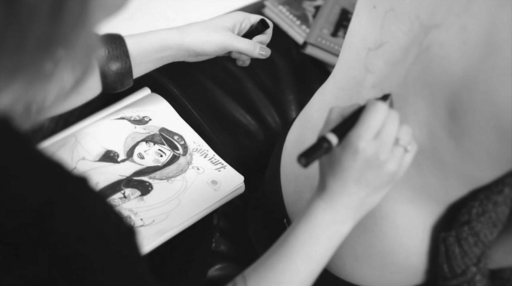
\includegraphics[width=0.4\textwidth]{samples/mrs.easy/101.png}}
{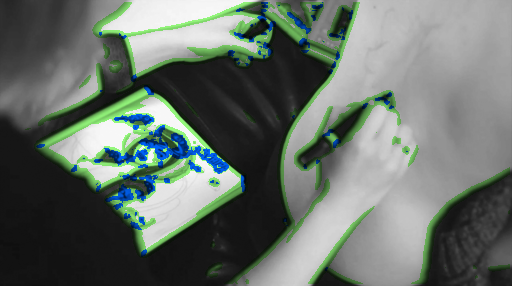
\includegraphics[width=0.4\textwidth]{u04.surf/harris_corner.png}}
\end{center}
\caption{Die Eingabebild und interessante Punkte nach Harris-Corner-Detection}
\label{fig:u04-picture}
\end{figure}

Mit Ausführen der Datei u04t08.m kann Harris-Corner Detektion durchgef\"uhrt werden.

\lstset{language=matlab}
\begin{lstlisting}[caption={Funktion f\"ur den Harris-Corner-Detector}]
% I - intensity image
% N - neighborhood size, has to be odd
% 
% returns a matrix of image dimension classifying each pixel M(y,x) as
% 0 - nothing
% 1 - edge
% 2 - corner
function M = detectCorners(I, N)
    if mod(N,2) == 0
        printf('unsupported neighborhood size in corner detector');
        return;
    endif
    
    [r c] = size(I);
    W = gaussmatrix(N,N/2);
    N2 = (N-1)/2;
    [Dr Dc] = gradient(I);
    M = zeros(r,c);
    
    for i=N2+1:r-N2
      for j=N2+1:c-N2
        % create window around current pixel (j,i)
        Ix = Dr((i-N2):(i+N2),(j-N2):(j+N2));
        Iy = Dc((i-N2):(i+N2),(j-N2):(j+N2));
    
        % see http://www.cse.yorku.ca/~kosta/CompVis_Notes/harris_detector.pdf
        % CAREFUL: this is not be the same corner detector as in the SURF-paper,
        % this is from the Harris-Paper
        S1 = sum(sum(Ix.^2 .* W));
        S2 = S3 = sum(sum(Ix.*Iy.*W)); 
        S4 = sum(sum(Iy.^2 .* W));
        C = [S1, S2 ; S3, S4];
        % is there any scaling possibility for better 'big lambda' decision?
        l = eig(C);
        % search for big eigenvalues, one big -> edge, two big -> corner 
        if bigLambda(l(1)) && bigLambda(l(2))
            M(i,j) = 2;
        elseif bigLambda(l(1)) || bigLambda(l(2))
            M(i,j) = 1;
        endif;
      endfor
    endfor
end

function ret = bigLambda(l)
    ret = l > 20;
end
\end{lstlisting}

Die Visualisierung erfolgt im HSV-Farbraum, wobei das urspr\"ungliche Bild
als H=0, S=0 und V=Intensit\"at kodiert wird. Der zugeordnete Typ (Kante, Ecke) wird
durch den Farbwert definiert:

\lstset{language=matlab}
\begin{lstlisting}[caption={Visualisierung der interessanten Punkte}]
C = detectCorners(I,5);

Out = zeros(rows, cols, 3);
Out(:,:,1) = C(:,:) .* 0.3; % Hue
Out(:,:,2) = C(:,:) .* 0.5; % Saturation
Out(:,:,3) = I(:,:) ./ 255; % Value

Out = hsv2rgb(Out);

imshow(Out);
\end{lstlisting}

\section*{Aufgabe 9 - SURF Deskriptor}

---

% \includegraphics[width=150mm]{<file.eps>}
\end{document}
